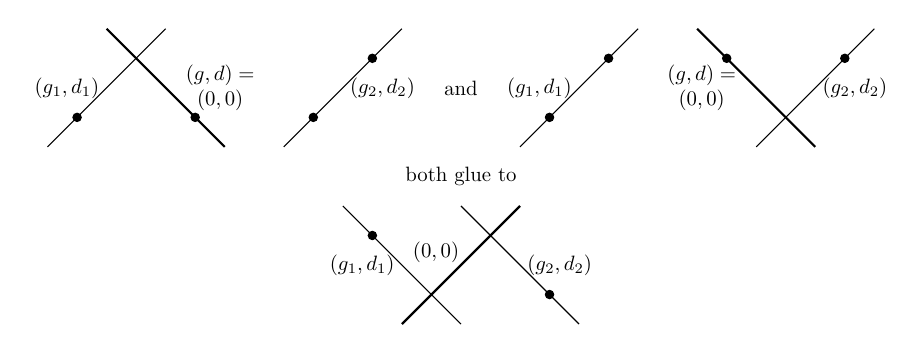
\begin{tikzpicture}[scale=.75,every node/.style={transform shape}]
  \draw (0,0) -- node[left]{$(g_1,d_1)$} (2,2);
  \draw[thick] (1,2) -- node[right]{\begin{tabular}{c} $(g,d)=$ \\ $(0,0)$ \end{tabular}} (3,0);
  \draw[fill=black] (.5,.5) circle[radius=2pt] (2.5,.5) circle[radius=2pt];
  \draw (4,0) -- node[right]{$(g_2,d_2)$}(6,2);
  \draw[fill=black] (4.5,.5) circle[radius=2pt] (5.5,1.5) circle[radius=2pt];
  
  \draw (7,1) node{and};
  
  \draw (8,0) -- node[left]{$(g_1,d_1)$} (10,2);
  \draw[fill=black] (8.5,.5) circle[radius=2pt] (9.5,1.5) circle[radius=2pt];
  \draw[thick] (11,2) -- node[left]{\begin{tabular}{c} $(g,d)=$ \\ $(0,0)$ \end{tabular}} (13,0);
  \draw (12,0) -- node[right]{$(g_2,d_2)$} (14,2);
  \draw[fill=black] (11.5,1.5) circle[radius=2pt] (13.5,1.5) circle[radius=2pt];

  \draw (7,-.5) node{both glue to};
  
  \draw (5,-1) -- node[left]{$(g_1,d_1)$}(7,-3) (7,-1) -- node[right]{$(g_2,d_2)$} (9,-3);
  \draw[thick] (6,-3) -- node[above left=-.1cm]{$(0,0)$} (8,-1);
  \draw[fill=black] (5.5,-1.5) circle[radius=2pt] (8.5,-2.5) circle[radius=2pt];
\end{tikzpicture}